%%%%%%%%%%%%%%%%%%%%%%%%%%%%%%%%%%%%%
%                                   %
% Compile with XeLaTeX and biber    %
%                                   %
% Questions or comments:            %
%                                   %
% joshua dot mcneill at uga dot edu %
%                                   %
%%%%%%%%%%%%%%%%%%%%%%%%%%%%%%%%%%%%%

\documentclass{beamer}
  % Read in standard preamble (cosmetic stuff)
  %%%%%%%%%%%%%%%%%%%%%%%%%%%%%%%%%%%%%%%%%%%%%%%%%%%%%%%%%%%%%%%%
% This is a standard preamble used in for all slide documents. %
% It basically contains cosmetic settings.                     %
%                                                              %
% Joshua McNeill                                               %
% joshua dot mcneill at uga dot edu                            %
%%%%%%%%%%%%%%%%%%%%%%%%%%%%%%%%%%%%%%%%%%%%%%%%%%%%%%%%%%%%%%%%

% Beamer settings
% \usetheme{Berkeley}
\usetheme{CambridgeUS}
% \usecolortheme{dove}
% \usecolortheme{rose}
\usecolortheme{seagull}
\usefonttheme{professionalfonts}
\usefonttheme{serif}
\setbeamertemplate{bibliography item}{}

% Packages and settings
\usepackage{fontspec}
  \setmainfont{Charis SIL}
\usepackage{hyperref}
  \hypersetup{colorlinks=true,
              allcolors=blue}
\usepackage{graphicx}
  \graphicspath{{../../figures/}}
\usepackage[normalem]{ulem}
\usepackage{enumerate}

% Document information
\author{M. McNeill}
\title[FREN2001]{Français 2001}
\institute{\url{joshua.mcneill@uga.edu}}
\date{}

%% Custom commands
% Lexical items
\newcommand{\lexi}[1]{\textit{#1}}
% Gloss
\newcommand{\gloss}[1]{`#1'}
\newcommand{\tinygloss}[1]{{\tiny`#1'}}
% Orthographic representations
\newcommand{\orth}[1]{$\langle$#1$\rangle$}
% Utterances (pragmatics)
\newcommand{\uttr}[1]{`#1'}
% Sentences (pragmatics)
\newcommand{\sent}[1]{\textit{#1}}
% Base dir for definitions
\newcommand{\defs}{../definitions}


  % Packages and settings
  \usepackage[backend=biber, style=apa]{biblatex}
    \addbibresource{../references/References.bib}

  % Document information
  \subtitle[Intro to Semantics]{Introduction to Semantics}

  %% Custom commands
  % Subsection/frame titles
  \newcommand{\suboneone}{What is it?}
  \newcommand{\subonetwo}{What do we mean by meaning?}
  \newcommand{\subtwoone}{Sense}
  \newcommand{\subtwotwo}{Reference}
  \newcommand{\subtwothree}{Sense relations}
  \newcommand{\subtwofour}{Practice}

\begin{document}
  % Read in the standard intro slides (title page and table of contents)
  %%%%%%%%%%%%%%%%%%%%%%%%%%%%%%%%%%%%%%%%%%%%%%%%%%%%%%%%%%%%%%%%
% This is a standard set of intro slides used in for all slide %
% documents. It basically contains the title page and table of %
% contents.                                                    %
%                                                              %
% Joshua McNeill                                               %
% joshua dot mcneill at uga dot edu                            %
%%%%%%%%%%%%%%%%%%%%%%%%%%%%%%%%%%%%%%%%%%%%%%%%%%%%%%%%%%%%%%%%

\begin{frame}
  \titlepage
  \tiny{Office: % Basically a variable for office hours location
Gilbert 121\\
        Office hours: % Basically a variable for office hours
 lundi, mercredi, vendredi 10:10--11:10
}
\end{frame}

\begin{frame}
  \tableofcontents[hideallsubsections]
\end{frame}

\AtBeginSection[]{
  \begin{frame}
    \tableofcontents[currentsection,
                     hideallsubsections]
  \end{frame}
}


  \section{Semantics Basics}
    \subsection{\suboneone}
      \begin{frame}{\suboneone}
        \begin{definition}
          % Semantics
The study of meaning

        \end{definition}
        \begin{example}<2->
          We said that \lexi{bank}\textsubscript{1} and \lexi{bank}\textsubscript{2} have unrelated meanings:
          \begin{itemize}
            \item How does that work?
            \item How do we model that?
          \end{itemize}
        \end{example}
      \end{frame}

      \begin{frame}{\suboneone}
        \begin{block}{What we're not talking about}
          Dictionaries
          \begin{itemize}
            \item Represent meanings that some group tends to agree on
            \item But, we're interested in meanings in individuals' languages
          \end{itemize}
        \end{block}
        \begin{example}<2->
          `There's a dearth of hoagies.'
          \begin{itemize}
            \item Is \lexi{dearth} many or few?
            \item What does \lexi{hoagie} bring to mind?
          \end{itemize}
        \end{example}
      \end{frame}

      \begin{frame}{\suboneone}
        \begin{block}{Two broad areas of semantics}
          \begin{itemize}
            \item Lexical semantics
            \item Compositional semantics
          \end{itemize}
        \end{block}
        \begin{alertblock}{Lexical semantics}
          % Lexical semantics
The area of semantics concerned with the meanings of lexical expressions

        \end{alertblock}
        \begin{alertblock}{Compositional semantics}
          % Compositional semantics
The area of semantics concerned with the meanings created through the combination of multiple lexical expressions

        \end{alertblock}
      \end{frame}

    \subsection{\subonetwo}
      \begin{frame}[t]{\subonetwo}
        \begin{block}{Two aspects of meaning}
          \begin{itemize}
            \item \alert{Sense}: % Sense
A meaning of a linguistic expression in terms of its relationship with the rest of the language of which it is part

            \item \alert{Reference}: % Reference
The connection between a linguistic expression and an object in the world

          \end{itemize}
        \end{block}
        \only<2>{
          \begin{example}
            The senses of \lexi{dog}:
            \begin{itemize}
              \item \lexi{pet}, \lexi{furry}, \lexi{four legs}, \lexi{mammal}, \lexi{companion}, \lexi{canine}, etc.
            \end{itemize}
          \end{example}
        }
        \only<3-4>{
          \begin{example}
            \parbox{0.48\linewidth}{
              The reference for \lexi{dog}:
              \begin{itemize}
                \item<4-> \alert{Referent}: % Referent
The thing in the world to which a linguistic expression is connected

              \end{itemize}
            }
            \parbox{0.48\linewidth}{
              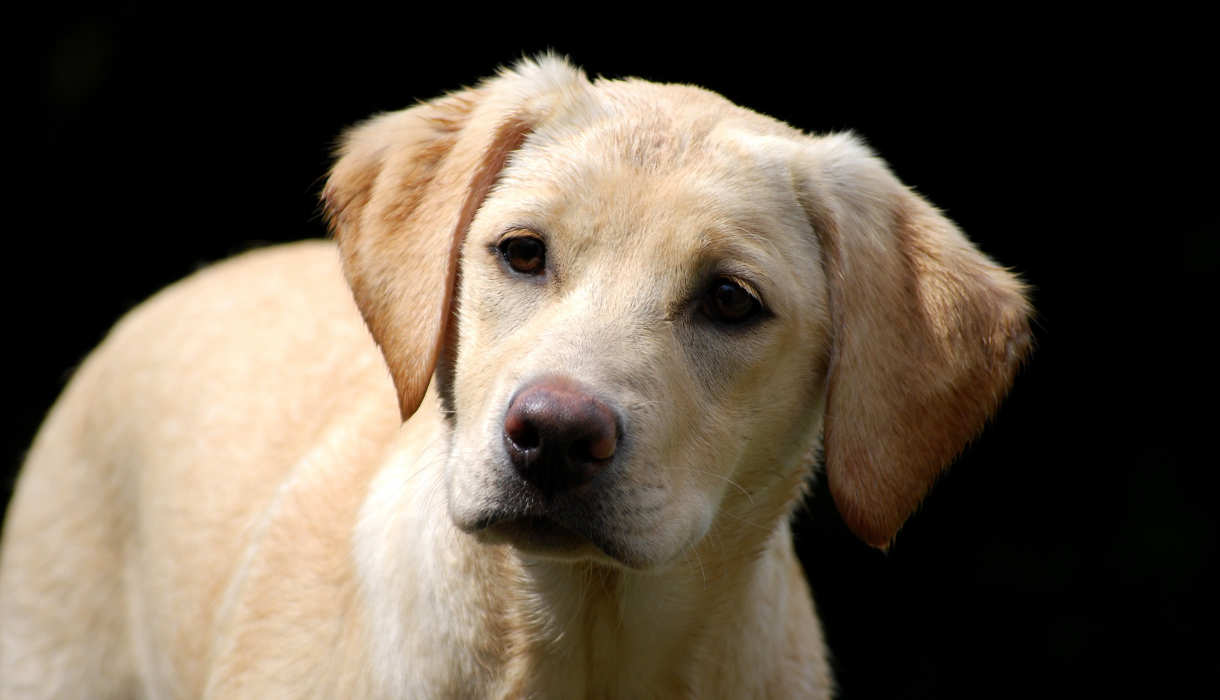
\includegraphics[scale=0.4]{dog.jpg}
            }
          \end{example}
        }
      \end{frame}

      % Things probably not to cover b/c they assume that meaning is not language (i.e., individual) dependent
        % They claim that knowing an expression's sense doesn't help with knowing its reference (e.g., diamond)
        % They claim that unicorn has no reference, just senses
        % They claim the same for Queen of the US

      % Also, this section is kinda weak as a point, so probably just skip
      % \begin{frame}{\subonetwo}
      %   \begin{center}
      %     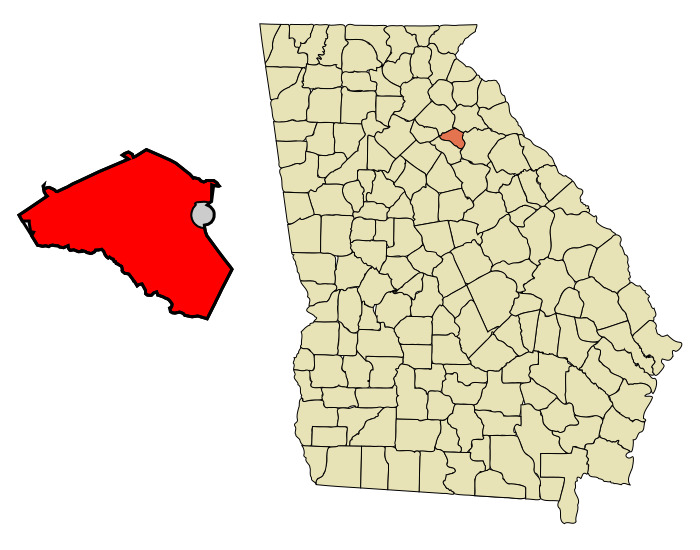
\includegraphics[scale=0.17]{athens.jpg}
      %   \end{center}
      %   \begin{columns}
      %     \column{0.5\linewidth}
      %       \begin{block}{\lexi{The city where R.E.M. got their start}}
      %         Senses:
      %         \begin{itemize}
      %           \item \lexi{Athens}, \lexi{Georgia}, \lexi{music}, \lexi{alternative}, etc.
      %         \end{itemize}
      %       \end{block}
      %     \column{0.5\linewidth}
      %       \begin{block}{\lexi{The city where the University of Georgia is located}}
      %         Senses:
      %         \begin{itemize}
      %           \item \lexi{Athens}, \lexi{Georgia}, \lexi{university}, etc.
      %         \end{itemize}
      %       \end{block}
      %   \end{columns}
      % \end{frame}

  \section{Lexical Semantics}
    \subsection{\subtwoone}
      \begin{frame}{\subtwoone}
        \begin{block}{}
          The concept of \lexi{sense} is pretty vague
        \end{block}
        \begin{block}{What senses might be linked to in your language}
          \begin{itemize}
            \item Other expressions
            \item Mental images
          \end{itemize}
        \end{block}
      \end{frame}

      \begin{frame}[t]{\subtwoone}
        \begin{block}{Linked to other expressions?}
          We do often talk about sense relations in semantics
          \begin{itemize}
            \item<2-> But, this can be circular
          \end{itemize}
        \end{block}
        \begin{example}
          Sense of \lexi{pride}:
          \begin{itemize}
            \item `The quality of state of being proud'
          \end{itemize}
          \uncover<2->{
            Sense of \lexi{proud}:
            \begin{itemize}
              \item `Feeling or showing pride'
            \end{itemize}
          }
        \end{example}
      \end{frame}

      \begin{frame}[t]{\subtwoone}
        \begin{block}{Linked to mental images?}
          This is useful and gets around any circularity
          \begin{itemize}
            \item<3-> But, how do we get to non-prototypes?
            \item<5-> This also encroaches on the concept of reference
            \item<6-> And what about words like \lexi{the} or \lexi{pride}?
          \end{itemize}
        \end{block}
        \begin{example}
          \parbox{0.48\linewidth}{
            Sense of \lexi{bird}:
            \begin{itemize}
              \item<2-> \alert{Prototype}: % Prototype
A typical or ideal mental image associated with a linguistic expression

            \end{itemize}
          }
          \parbox{0.48\linewidth}{
            \only<-2>{
              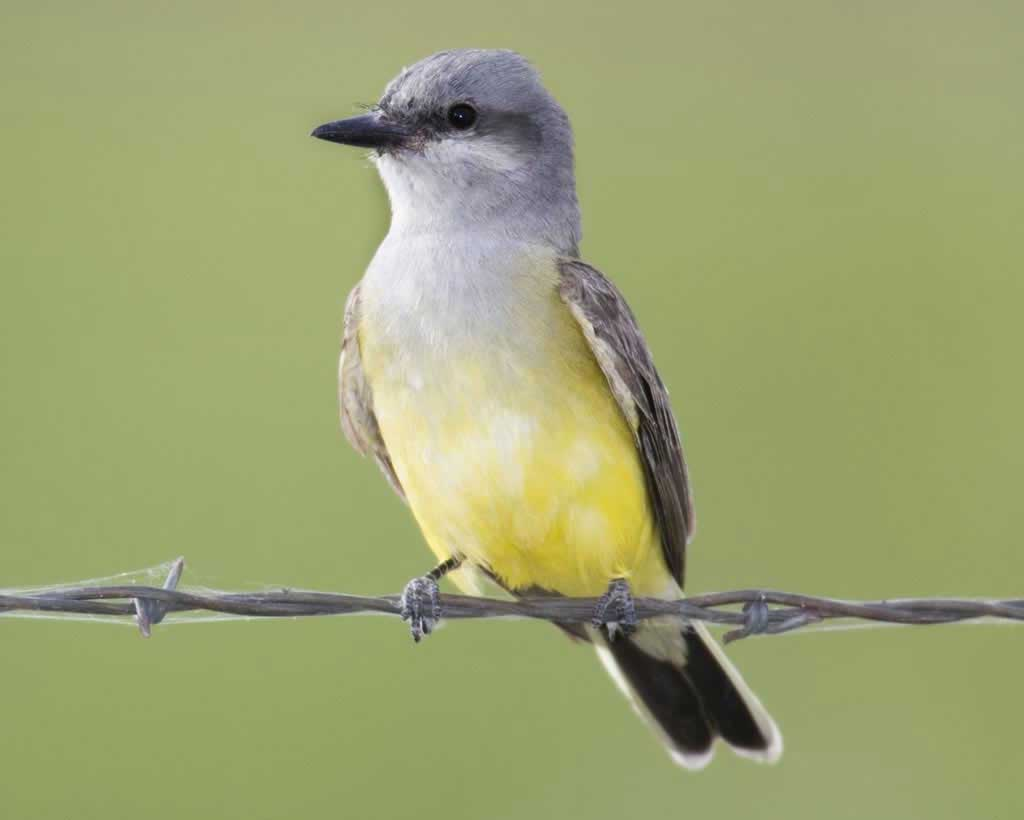
\includegraphics[scale=0.08]{bird_proto.jpg}
            }
            \only<3>{
              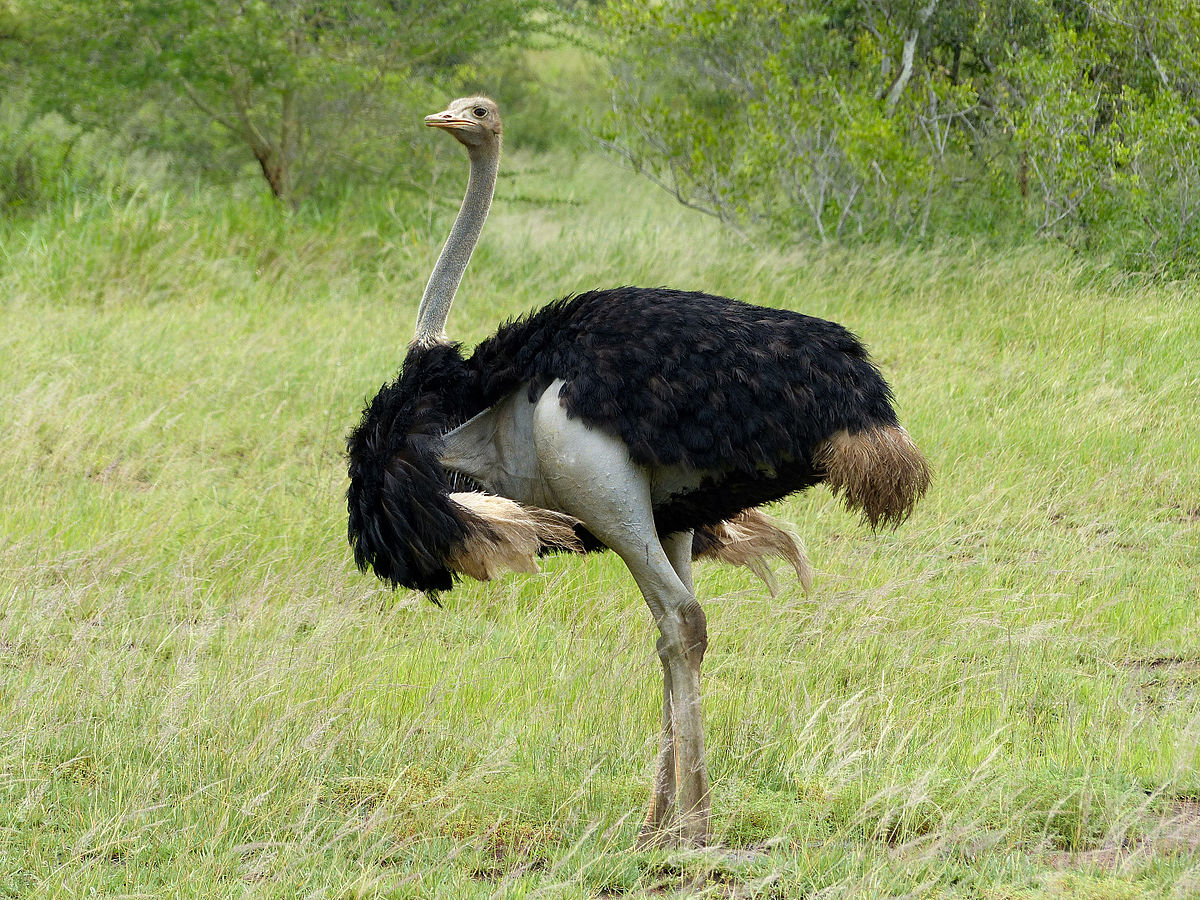
\includegraphics[scale=0.075]{bird_ostrich.jpg}
            }
            \only<4->{
              
\includegraphics[scale=0.06]{bird_penguin.jpg}
            }
          }
        \end{example}
      \end{frame}

      \begin{frame}{\subtwoone}
        \begin{block}{}
          In this class, we'll typically talk about sense as connections between different expressions
        \end{block}
      \end{frame}

    \subsection{\subtwotwo}
      \begin{frame}{\subtwotwo}
        \begin{block}{}
          Reference is clearer than sense
        \end{block}
        \begin{block}{Lexical categories we'll look at}
          \begin{itemize}
            \item Proper nouns
            \item Common nouns
            \item Non-nouns
          \end{itemize}
        \end{block}
      \end{frame}

      \begin{frame}[t]{\subtwotwo}
        \begin{block}{Proper nouns}
          Simple, because reference is to exactly one thing
        \end{block}
        \begin{columns}
          \column{0.48\linewidth}
            \begin{minipage}[c][0.6\textheight]{\linewidth}
              \begin{block}{}
                \begin{itemize}
                  \item \lexi{China}:
                  \item<2-> \lexi{Dr. John}:
                  \item<3-> \lexi{Sanford Stadium}:
                \end{itemize}
              \end{block}
            \end{minipage}
          \column{0.48\linewidth}
            \only<1>{
              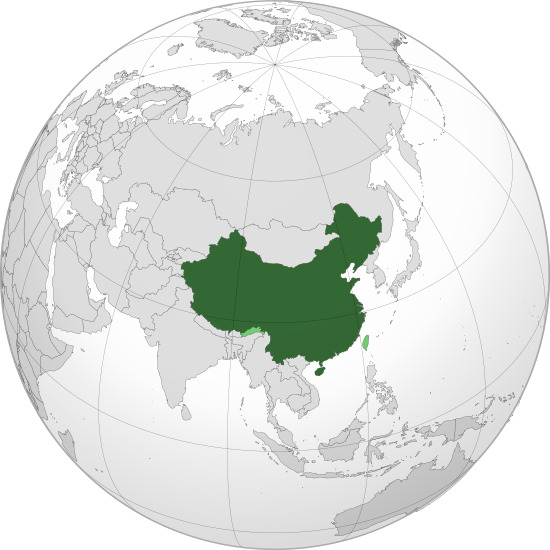
\includegraphics[scale=0.2]{china.jpg}
            }
            \only<2>{
              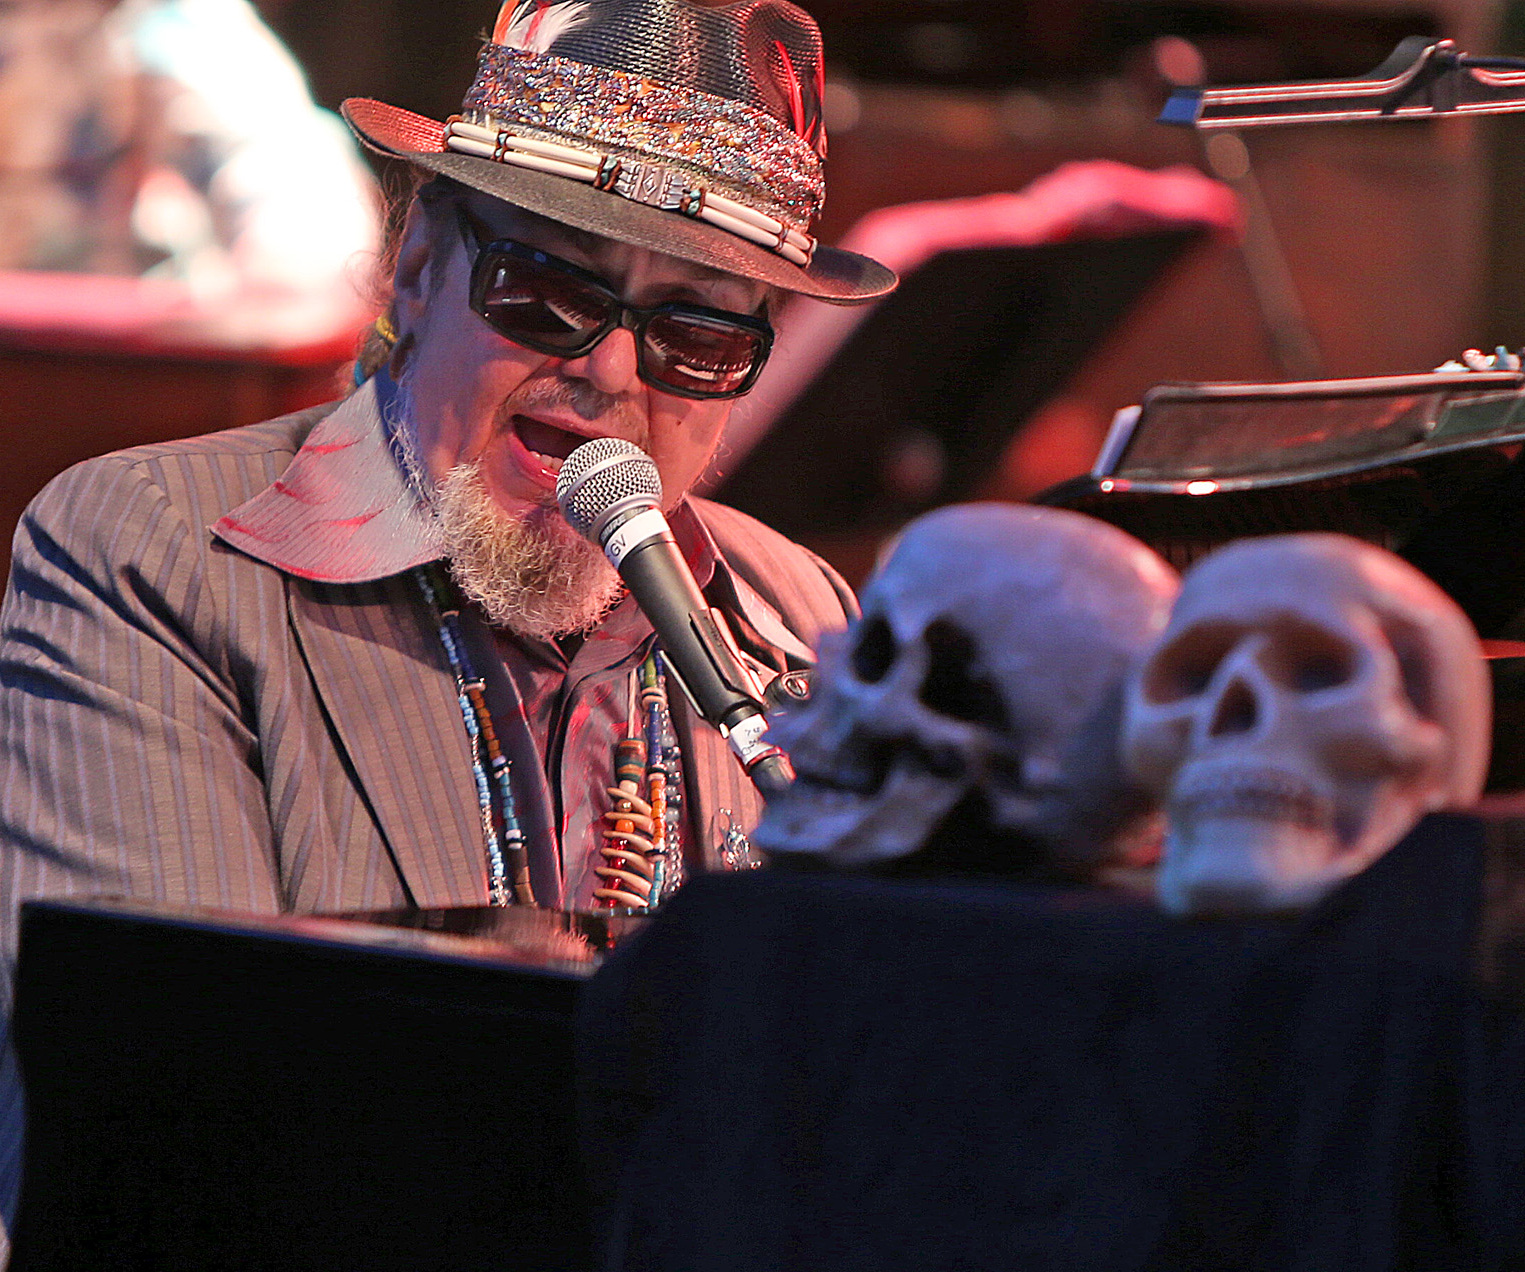
\includegraphics[scale=0.25]{dr_john.jpg}
            }
            \only<3>{
              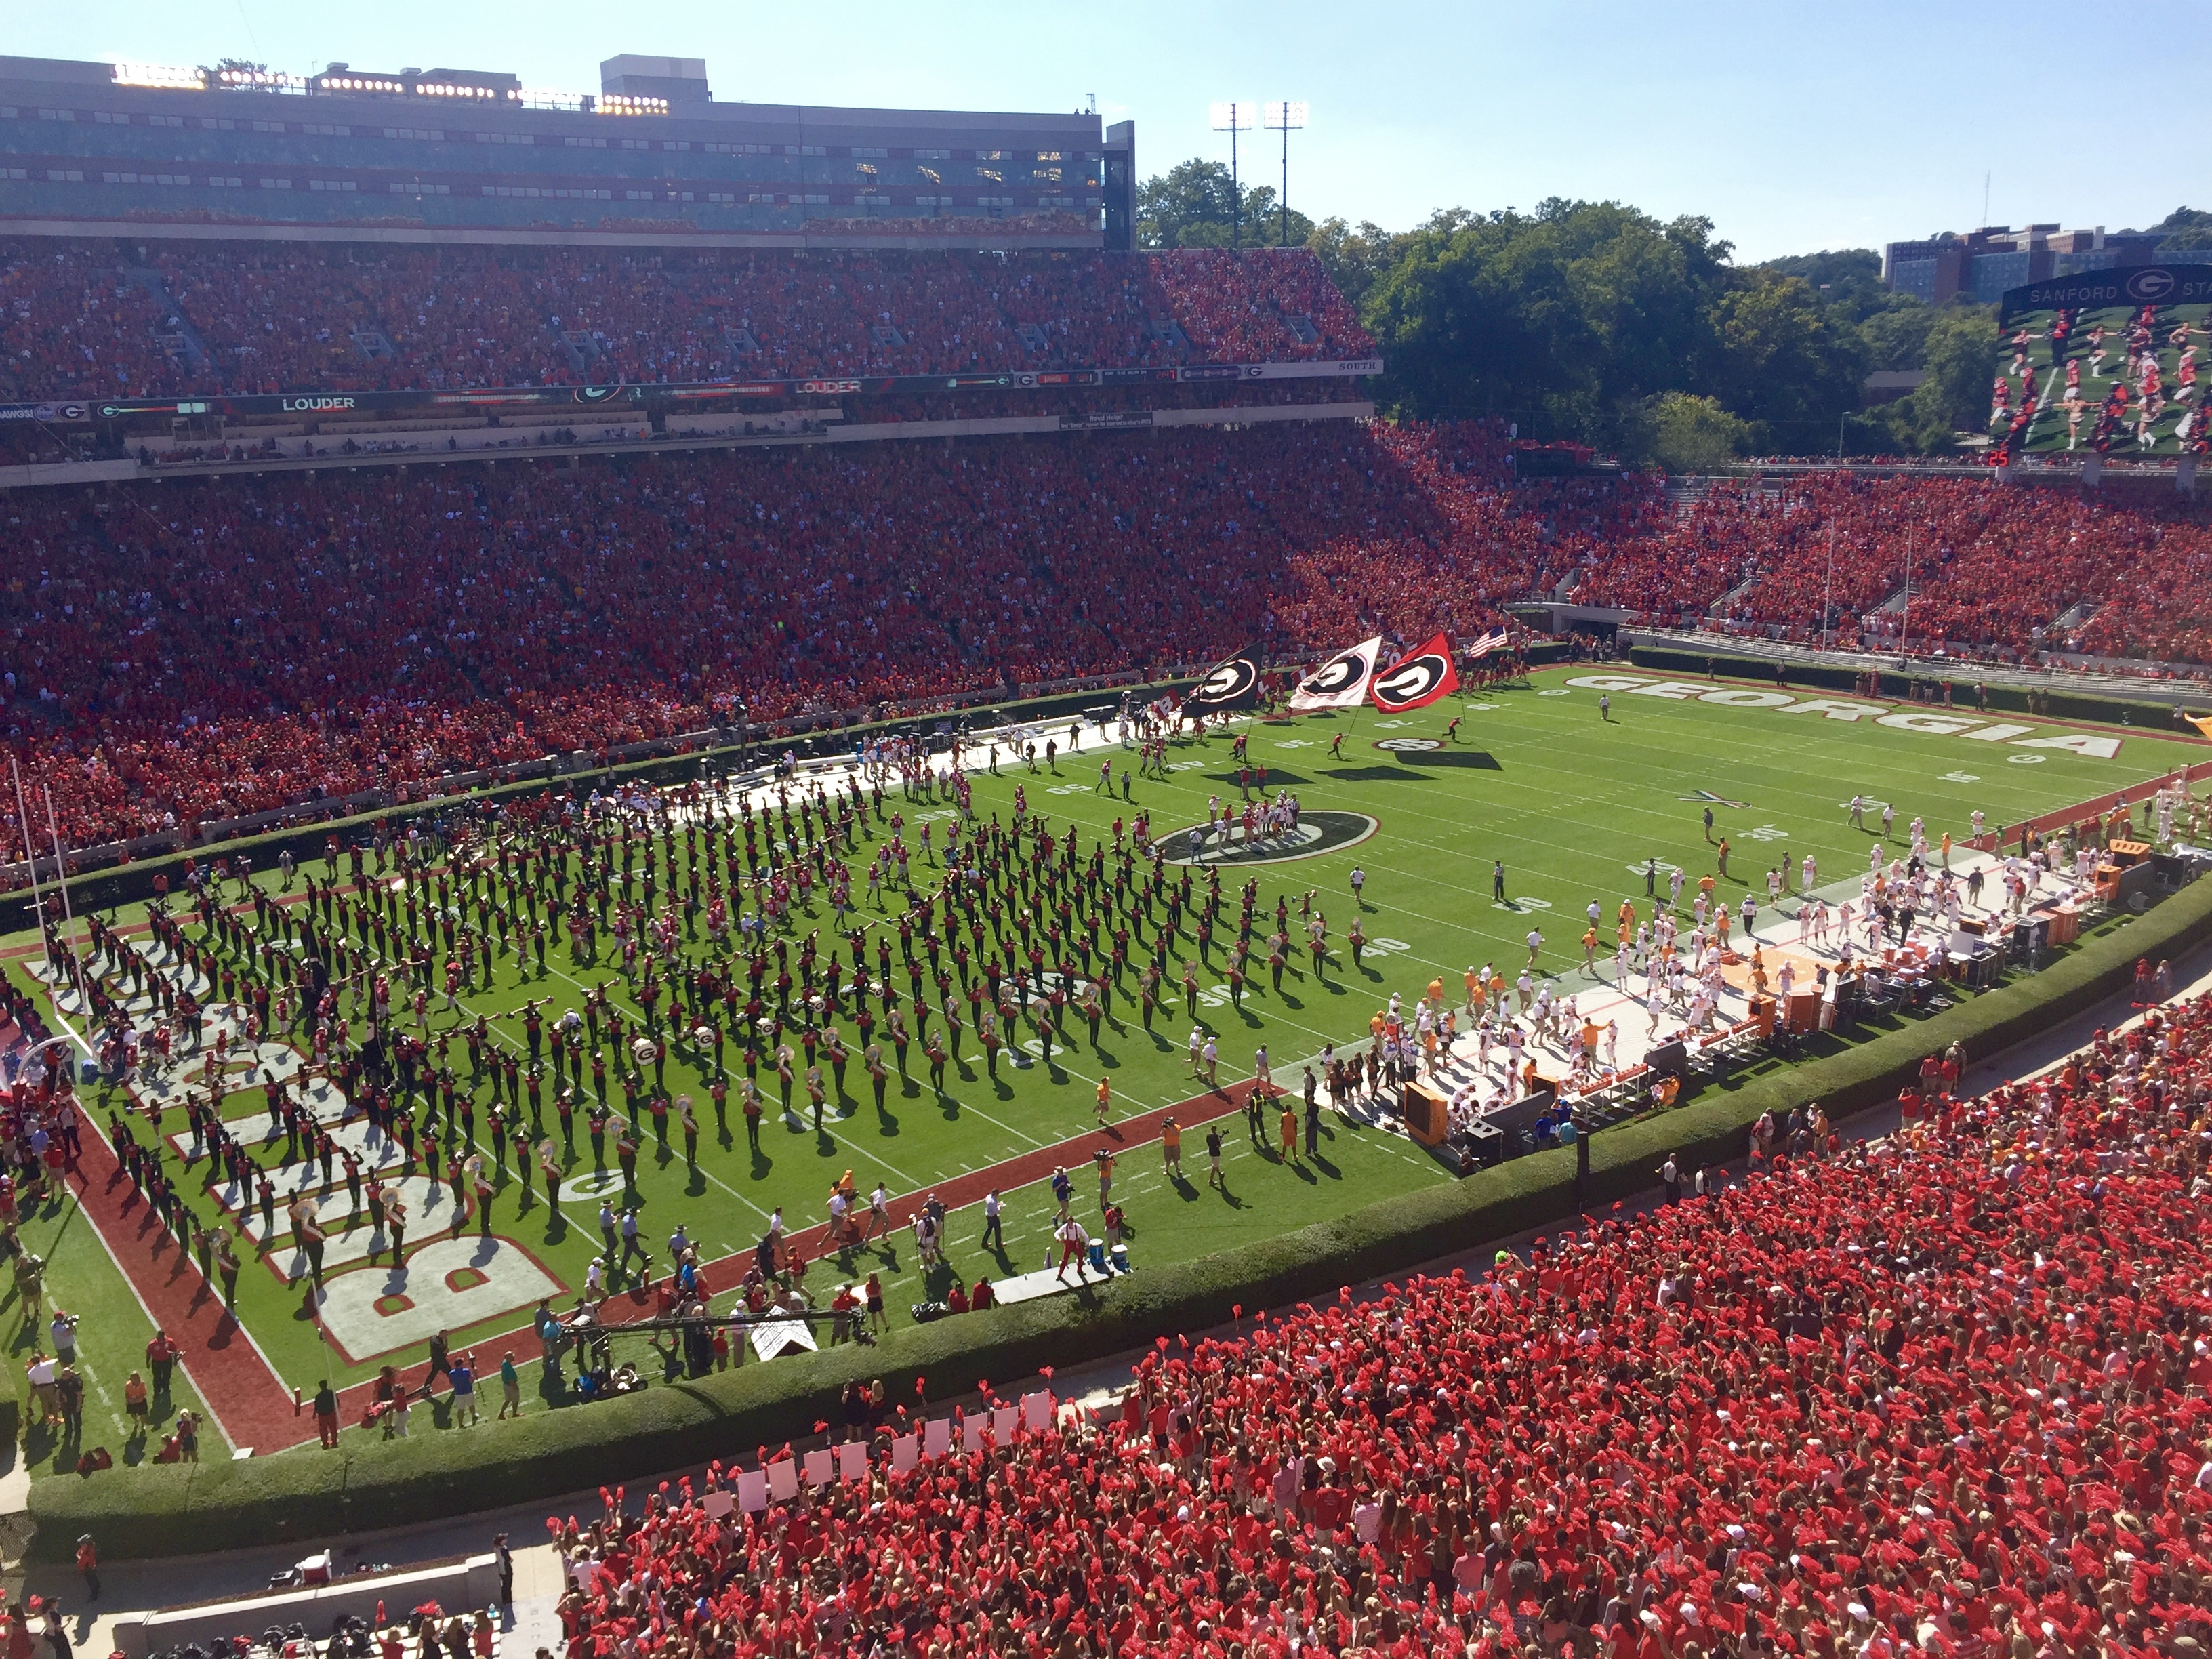
\includegraphics[scale=0.042]{sanford_stadium.jpg}
            }
        \end{columns}
      \end{frame}

      \begin{frame}[t]{\subtwotwo}
        \begin{block}{Common nouns}
          Reference is to a set of things
        \end{block}
        \begin{block}{}
          \begin{itemize}
            \item \lexi{A cat}:
            \item<2-> \lexi{A woman}:
          \end{itemize}
        \end{block}
        \begin{center}
          \only<1>{
          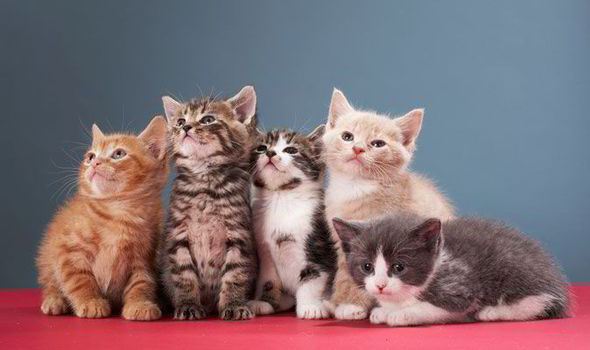
\includegraphics[scale=0.25]{cats.jpg}
          }
          \only<2>{
          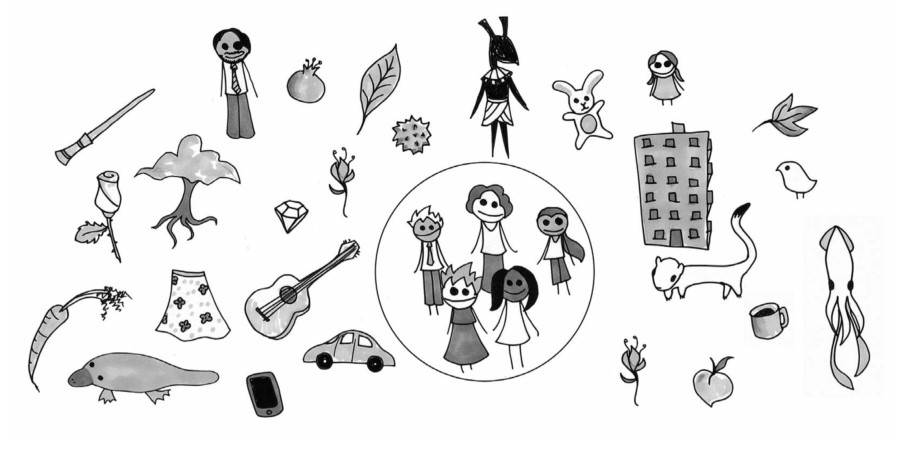
\includegraphics[scale=0.4]{women.jpg}
          }
        \end{center}
      \end{frame}

      \begin{frame}[t]{\subtwotwo}
        \begin{block}{Non-nouns}
          Reference works when they can be expressed as nouns
        \end{block}
        \begin{columns}
          \column{0.48\linewidth}
            \begin{minipage}[c][0.6\textheight]{\linewidth}
              \begin{block}{}
                \begin{itemize}
                  \item \lexi{Swim} (V):
                  \item<2-> \lexi{Purple} (Adj):
                \end{itemize}
              \end{block}
            \end{minipage}
          \column{0.48\linewidth}
            \only<1>{
              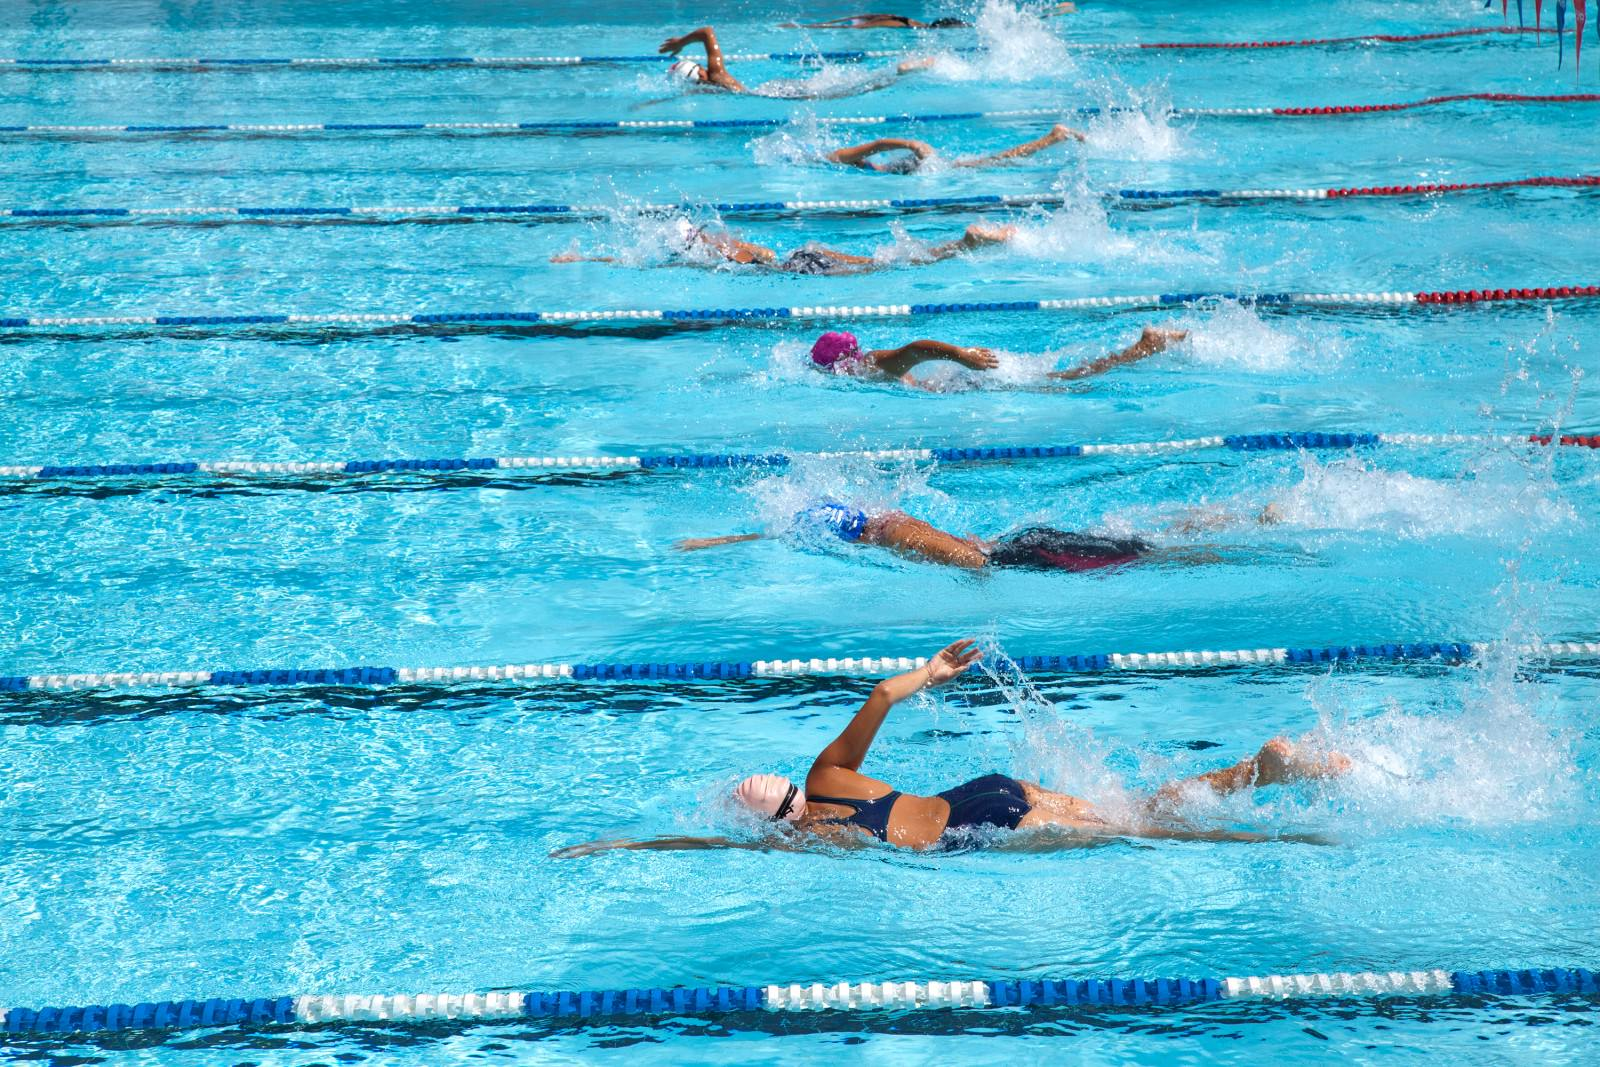
\includegraphics[scale=0.082]{swim.jpg}
            }
            \only<2>{
              
\includegraphics[scale=0.175]{purple.jpg}
            }
        \end{columns}
      \end{frame}

    \subsection{\subtwothree}
      \begin{frame}{\subtwothree}
        \begin{block}{Which two words seem more related?}
          \begin{itemize}
            \item \alert<2->{\lexi{Pot}}
            \item \lexi{Floor}
            \item \alert<2->{\lexi{Pan}}
          \end{itemize}
        \end{block}
        \begin{alertblock}<2->{Sense relation}
          % Sense relation
The type of a sense connection between two expressions

        \end{alertblock}
        \begin{block}<2->{The types}
          \begin{itemize}
            \item Hyponymy
            \item Synonymy
            \item Antonymy
          \end{itemize}
        \end{block}
      \end{frame}

      \begin{frame}[t]{\subtwothree}
        \begin{alertblock}{Hyponymy}
          % Hyponymy
A sense relation in which one expression's sense is a more restricted version of some other's

          \only<1>{
            \begin{itemize}
              \item \alert{Hyponym}: % Hyponym
An expression whose sense is a more restricted version of some other's

              \item \alert{Hypernym}: % Hypernym
An expression whose sense is a more general version of some other's

            \end{itemize}
          }
        \end{alertblock}
        \begin{columns}
          \column{0.48\linewidth}
            \begin{minipage}[c][0.6\textheight]{\linewidth}
              \begin{example}<2->
                \only<2-3>{
                  \begin{itemize}
                    \item \lexi{Poodle} is a hyponym of \lexi{dog}
                    \item<3-> Multiple layers are possible
                  \end{itemize}
                }
                \only<4->{
                  \lexi{Dog}, \lexi{sheep}, \lexi{cow}, and \lexi{platypus} are \alert{sister terms}:
                  \begin{itemize}
                    \item % Sister terms
A set of expressions that all share the same hypernym

                  \end{itemize}
                }
              \end{example}
            \end{minipage}
          \column{0.48\linewidth}
            \only<2>{
              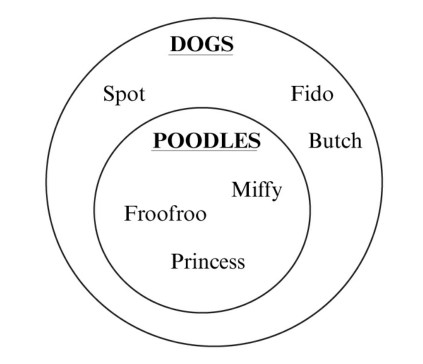
\includegraphics[scale=0.6]{dogs_poodles.jpg}
            }
            \only<3->{
              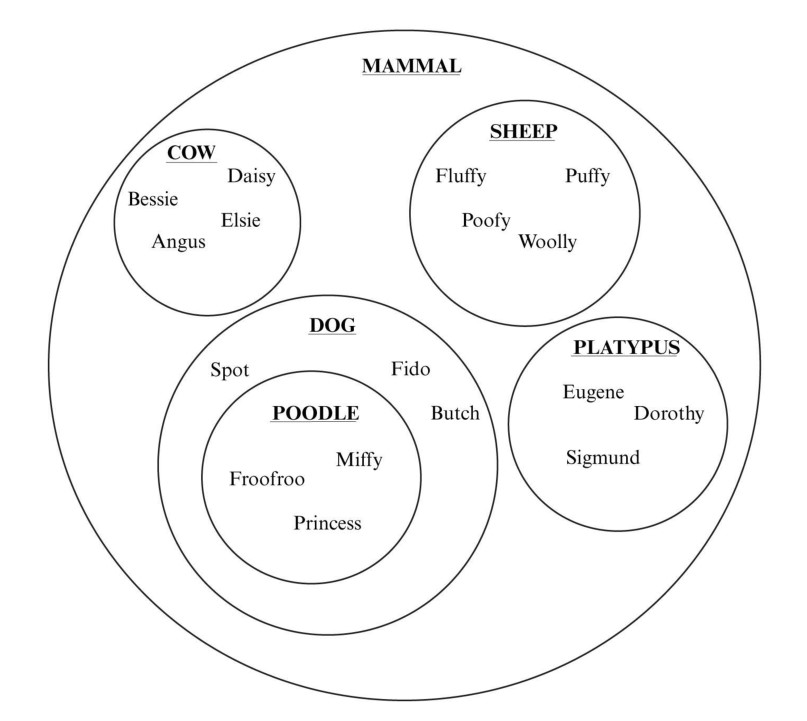
\includegraphics[scale=0.325]{dogs_mammals.jpg}
            }
        \end{columns}
      \end{frame}

      \begin{frame}[t]{\subtwothree}
        \begin{alertblock}{Synonymy}
          % Synonymy
A sense relation in which one expression's sense is the same as another's

        \end{alertblock}
        \begin{example}<2->
          True examples are rare: e.g., \lexi{couch} and \lexi{sofa}
          \begin{itemize}
            \item<3-> \lexi{Sofa} might sound more British
            \item<3-> \lexi{Sofa} might sound more formal
            \item<3-> \lexi{Sofa} might be for a living room and \lexi{couch} a family room
          \end{itemize}
        \end{example}
      \end{frame}

      \begin{frame}[t]{\subtwothree}
        \begin{alertblock}{Antonymy}
          % Antonymy
A sense relation in which one expression's sense is the opposite of another's

        \end{alertblock}
        \begin{block}{`Opposite' is vague}
          So we'll talk about types of opposites:
          \begin{itemize}
            \item Complementary antonyms
            \item Gradable antonyms
            \item Reverse antonyms
            \item Converse antonyms
          \end{itemize}
        \end{block}
      \end{frame}

      \begin{frame}[t]{\subtwothree}
        \begin{alertblock}{Complementary antonyms}
          % Complementary antonyms
A pair of expressions whose senses are opposite in that, together, they exhaust all possibilities for what they describe

        \end{alertblock}
        \begin{columns}
          \column{0.48\linewidth}
            \begin{example}
              \begin{itemize}
                \item \lexi{off}/\lexi{on}
                \item \lexi{mortal}/\lexi{immortal}
                \item<2-> \lexi{dead}/\lexi{alive}
              \end{itemize}
            \end{example}
          \column{0.48\linewidth}
            \uncover<2->{
              
\includegraphics[scale=0.275]{dead_alive.jpg}
            }
        \end{columns}
      \end{frame}

      \begin{frame}[t]{\subtwothree}
        \begin{alertblock}{Gradable antonyms}
          % Gradable antonyms
A pair of expressions whose senses are opposite in that they are at opposite ends of a continuum of senses

        \end{alertblock}
        \begin{example}
          \begin{itemize}
            \item \lexi{wet}/\lexi{dry}
            \item \lexi{easy}/\lexi{hard}
            \item \lexi{young}/\lexi{old}
            \item \lexi{hot}/\lexi{cold}
          \end{itemize}
        \end{example}
      \end{frame}

      \begin{frame}{\subtwothree}
        \begin{block}{To distinguish between complementary and gradable antonyms:}
          \begin{itemize}
            \item Is there an expression with a sense in between?
            \item<2-> Can the question `how X?' be answered?
          \end{itemize}
        \end{block}
        \begin{example}
          \begin{enumerate}
            \item \lexi{dead}/\lexi{alive}?
            \item \lexi{young}/\lexi{old}?
            \item<2-> How \lexi{hot} is it?
            \item<2-> How \lexi{married} is he?
          \end{enumerate}
        \end{example}
      \end{frame}

      \begin{frame}[t]{\subtwothree}
        \begin{alertblock}{Reverse antonyms}
          % Reverse antonyms
A pair of expressions whose senses are opposite in that they describe actions that undo each other

        \end{alertblock}
        \begin{example}
          \begin{itemize}
            \item \lexi{expand}/\lexi{contract}
            \item \lexi{ascent}/\lexi{descent}
            \item \lexi{put together}/\lexi{take apart}
          \end{itemize}
        \end{example}
      \end{frame}

      \begin{frame}[t]{\subtwothree}
        \begin{alertblock}{Converse antonyms}
          % Converse antonyms
A pair of expressions whose senses are opposite in that one entails the existence of the other from a different point of view

        \end{alertblock}
        \begin{example}
          \begin{itemize}
            \item \lexi{lend}/\lexi{borrow}
            \item \lexi{send}/\lexi{receive}
            \item \lexi{over}/\lexi{under}
          \end{itemize}
        \end{example}
      \end{frame}

    \subsection{\subtwofour}
      \begin{frame}{\subtwofour}
        \begin{block}{Try these}
          \textcite{dawson_language_2016}, chapter 6 exercises 5, 8, 9, 10, and 12
        \end{block}
      \end{frame}

\end{document}
